\documentclass[final]{beamer}
\usepackage{hyperref,xspace,graphicx,microtype,minted,multicol,mflogo,enumerate,mathtools,hologo}
\usepackage[brazil]{babel}

\usetheme[sectionpage=simple,numbering=none]{metropolis}
\beamertemplatenavigationsymbolsempty

\newcommand{\filename}[1]{\texttt{#1}}
\newcommand{\code}[1]{\texttt{#1}}

\title{Introdução ao \LaTeX: sobre ombros de gigantes}
\author{Rafael Beraldo}
\date{28 de maio de 2016}

\begin{document}
\maketitle

\begin{frame}[standout]
  \Huge História
\end{frame}

\begin{frame}[plain]
  \begin{figure}[h]
    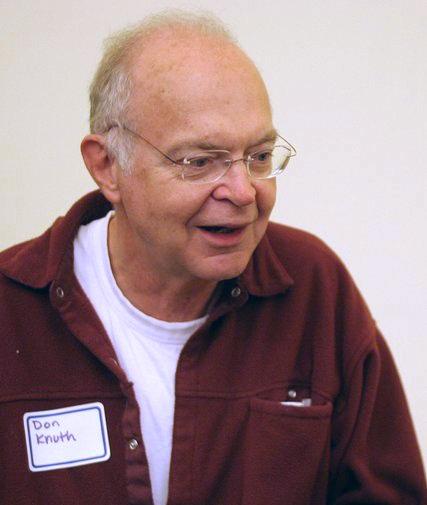
\includegraphics[scale=.5]{imagens/knuth}
    \caption{Donald Knuth em 2005}
  \end{figure}
\end{frame}

\begin{frame}[plain]
  \hspace*{-11.5mm}
  \begin{centering}
    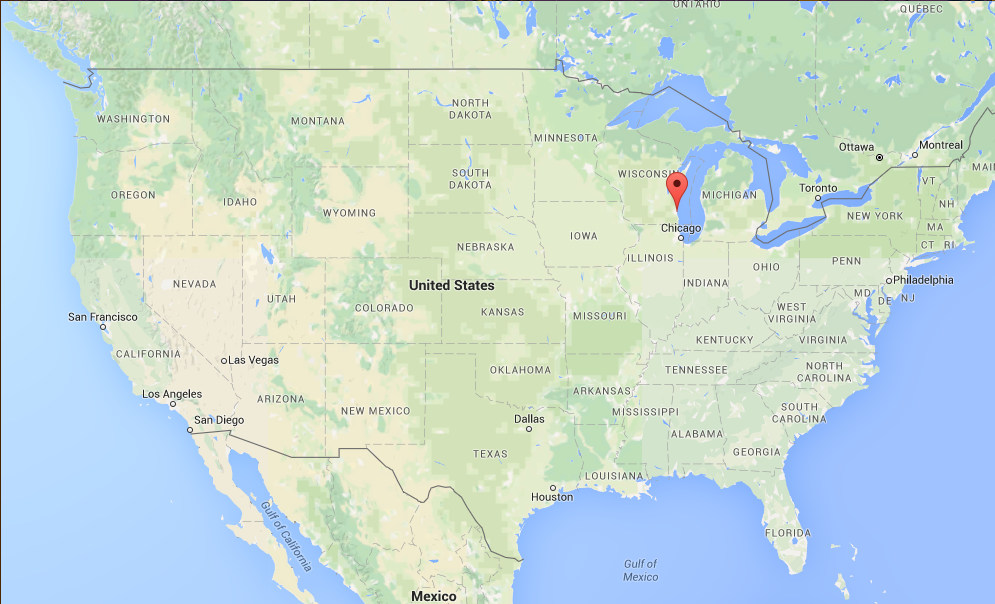
\includegraphics[width=\pagewidth]{imagens/milwaukee}
  \end{centering}
\end{frame}

\begin{frame}
  \Huge
  \only<1>{O pai de Knuth tinha uma editora}
  \only<2>{1977: segunda edição do segundo volume de \emph{The Art of Computer
  Programming}}
  \only<3>{\textsc{ascii} não foi projetado com livros em mente}
  \only<4>{\TeX: tau epsilon chi}
\end{frame}

\begin{frame}
  \large
  \begin{quote}
    The purpose of this pronunciation exercise is to remind you that \TeX\ is
    primarily concerned with high-quality technical manuscripts: Its emphasis
    is on art and technology, as in the underlying Greek word. If you merely
    want to produce a passably good document—something acceptable and basically
    readable but not really beautiful—a simpler system will usually suffice.
    With \TeX\ the goal is to produce the finest quality; this requires more
    attention to detail, but you will not find it much harder to go the extra
    distance, and you’ll be able to take special pride in the finished
    product.\hfill (Donald Knuth, \emph{\TeX book})
  \end{quote}
\end{frame}

\begin{frame}
  \Huge
  \LaTeX: 1985
\end{frame}

\begin{frame}[plain]
  \begin{figure}[h]
    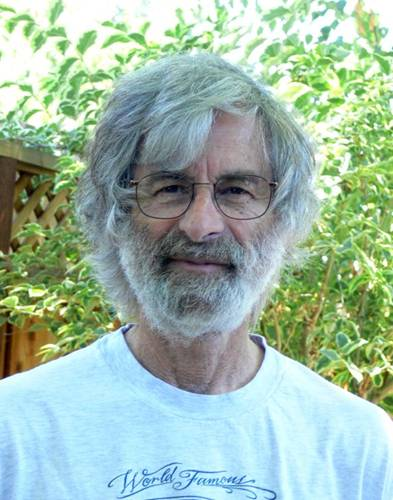
\includegraphics[scale=.5]{imagens/lamport}
    \caption{Leslie Lamport}
  \end{figure}
\end{frame}

\begin{frame}[standout]
  \Huge Filosofia
\end{frame}

% Considerações iniciais
\begin{frame}
  \only<1>{\Huge\LaTeX{} é uma linguagem de marcação de texto}
  \only<2>{\Huge Você \emph{declara} o documento}
  \only<3>{\Huge É como um tipógrafo profissional à sua disposição}
  \only<4>{\Huge Comandos são semânticos}
\end{frame}

% Sintaxe dos comandos
\begin{frame}[fragile]
  \begin{minted}[autogobble,fontsize=\huge,breaklines]{latex}
    \section{Introdução}
  \end{minted}
\end{frame}

% hello-world.tex %%%%%%%%%%%%%
\begin{frame}[standout]
  \huge
  \filename{hello-world.tex}
\end{frame}

\begin{frame}[fragile]
  \frametitle{\filename{hello-world.tex}}
  \begin{minted}[autogobble,fontsize=\Large,breaklines]{latex}
    \documentclass{article}
    \begin{document}
      Hello, world!
    \end{document}
  \end{minted}
\end{frame}

\begin{frame}[fragile]
  \frametitle{\filename{hello-world.tex}}
  \begin{minted}[autogobble,fontsize=\LARGE,breaklines]{bash}
    lualatex hello-world.tex
  \end{minted}
\end{frame}

\begin{frame}[fragile]
  \frametitle{\filename{hello-world.tex}}
  \begin{minted}[autogobble,breaklines]{latex}
    % hello-world.tex
    %
    % Rafael Beraldo <rberaldo@cabaladada.org>
    % Workshop de LaTeX do Opensanca
    % 28 de maio de 2016
  \end{minted}
\end{frame}

% Vamos cometer uns erros de propósito e lidar com as consequências?
\begin{frame}
  \frametitle{\filename{hello-world.tex}}
  \Huge
  Erros de compilação
\end{frame}

% simbolos-reservados.tex %%%%%%%%%%%%%%
\begin{frame}[standout]
  \Huge
  \filename{simbolos-reservados.tex}
\end{frame}

% Os símbolos a seguir são reservados e devem ser escapados:
\begin{frame}[fragile]
  \frametitle{\filename{simbolos-reservados.tex}}
  \begin{minted}[autogobble,fontsize=\LARGE,breaklines]{latex}
    # $ % ^ & _ { } ~ \

    \# \$ \% \^{} \& \_ \{ \} \~{} \textbackslash
  \end{minted}
\end{frame}

% Exercício: escapar os símbolos especiais até que o código compile
\begin{frame}
  \frametitle{\filename{simbolos-reservados.tex}}
  \Huge
  Resolver: \filename{simbolos-reservados.tex}
\end{frame}

% espaco-branco.tex %%%%%%%%%%%%%%
% No exemplo, temos dois parágrafos do Guia do Mochileiro das Galáxias.
\begin{frame}[standout]
  \Huge
  \filename{espaco-branco.tex}
\end{frame}

% Ensinar que, para criar uma nova linha, usamos estes comandos.
\begin{frame}[fragile]
  \frametitle{\filename{espaco-branco.tex}}
  \begin{minted}[autogobble,fontsize=\LARGE,breaklines]{latex}
    \\newline

    \\
  \end{minted}
\end{frame}

% Mostrar a extensão dos exercícios; pedir que o resolvam. Mostrar como os
% comentários contém as instruções.
\begin{frame}
  \frametitle{\filename{espaco-branco-exercicio.tex}}
  \LARGE
  Resolver \filename{espaco-branco-exercicio.tex}
\end{frame}

% poliglota-exercicio.tex %%%%%%%%%%%%%%
\begin{frame}[standout]
  \huge
  \filename{poliglota-exercicio.tex}
\end{frame}

% No exemplo anterior, espaco-branco.tex, os acentos — na verdade, % diacríticos — não apareceram. Alguém saberia o motivo?
\begin{frame}
  \frametitle{\filename{poliglota-exercicio.tex}}
  \huge
  Acentos não apareciam em \filename{espaco-branco.tex}
\end{frame}

% Para resolver, teremos que usar pacotes
\begin{frame}
  \frametitle{\filename{poliglota-exercicio.tex}}
  \Huge
  Solução: pacotes
\end{frame}

% Para carregar pacotes, usamos esta sintaxe
\begin{frame}[fragile]
  \frametitle{\filename{poliglota-exercicio.tex}}
  \begin{minted}[autogobble,fontsize=\LARGE,breaklines]{latex}
    \usepackage[opções]{pacote}
  \end{minted}
\end{frame}

% Para resolvermos a falta de diacríticos, usaremos o pacote polyglossia
\begin{frame}
  \frametitle{\filename{poliglota-exercicio.tex}}
  \Huge
  Pacote \code{polyglossia}
\end{frame}

\begin{frame}
  \frametitle{\filename{poliglota-exercicio.tex}}
  \Huge
  O \code{polyglossia} traz benefícios como:
  \begin{itemize}
    \only<1>{\item Hifenização}
    \only<2>{\item Strings como \mintinline{latex}{\today}}
    \only<3>{\item Convenções tipográficas localizadas}
  \end{itemize}
\end{frame}

% Ao exercício.
%
% Sabemos para que serve o polyglossia. Perguntar como ele seria implementado,
% e onde seria colocado no código.
%
% Também estudar a sintaxe para selecionar línguas. Explicar o motivo pelo qual
% a opção de pacote [brazil] não é mais usada: fica difícil selecionar várias
% línguas e suas opções.
\begin{frame}
  \frametitle{\filename{poliglota-exercicio.tex}}
  \Huge
  Como carregar o pacote \code{polyglossia}?
\end{frame}

\begin{frame}[fragile]
  \frametitle{\filename{poliglota-exercicio.tex}}
  \begin{minted}[autogobble,fontsize=\Large,breaklines]{latex}
    \usepackage{polyglossia}
    \setdefaultlanguage{brazil}
  \end{minted}
\end{frame}

% Para encontrar ajuda, podemos ler a documentação oficial dos pacotes que
% estamos usando. Mostrar outras opções do polyglossia, por exemplo.
\begin{frame}
  \frametitle{\filename{poliglota-exercicio.tex}}
  \Huge
  Comprehensive \TeX{} Archive Network

  \url{ctan.org}
\end{frame}

\begin{frame}
  \frametitle{\filename{poliglota-exercicio.tex}}
  \huge
  \url{https://www.ctan.org/pkg/polyglossia}
\end{frame}

% artigo.tex %%%%%%%%%%%%%%
\begin{frame}[standout]
  \huge
  \filename{artigo.tex}
\end{frame}

% Dar uma olhada no arquivo. Ensinar a distinção entre o preâmbulo e o corpo do
% documento.
\begin{frame}
  \frametitle{\filename{artigo.tex}}
  \LARGE
  Exemplo de arquivo comum em \LaTeX: \filename{artigo.tex}
\end{frame}

% Explicar as opções da classe article que escolhi
\begin{frame}[fragile]
  \frametitle{\filename{artigo.tex}}
  \huge
  Classes comuns:
  \begin{multicols}{2}
    \begin{itemize}
      \item\code{article}
      \item\code{report}
      \item\code{book}
      \item\code{letter}
      \item\code{memoir}
      \item\code{beamer}
  \end{itemize}
\end{multicols}
\end{frame}

% Vejamos quais são as opções de classe mais comuns
\begin{frame}
  \frametitle{\filename{artigo.tex}}
  \LARGE
  Opções de classe comuns:
  \begin{itemize}
    \only<1>{\item \code{10pt, 11pt, 12pt}}
    \only<1>{\item \code{a4paper, a5paper, letterpaper, …}}
    \only<1>{\item \code{fleqn}}
    \only<2>{\item \code{leqno}}
    \only<2>{\item \code{titlepage, notitlepage}}
    \only<2>{\item \code{twocolumn}}
    \only<2>{\item \code{twoside, oneside}}
    \only<3>{\item \code{landscape}}
    \only<3>{\item \code{openright, openany}}
    \only<3>{\item \code{draft}}
  \end{itemize}
\end{frame}

% Compilar o documento várias vezes, com opções diferentes
\begin{frame}
  \frametitle{\filename{artigo.tex}}
  \Huge
  Testar diferentes opções de classe
\end{frame}

% Olharemos agora os pacotes carregados
\begin{frame}
  \frametitle{\filename{artigo.tex}}
  \Huge
  Pacotes: \code{polyglossia, blindtext} e \code{hyperref}
\end{frame}

% Mudar o comando author para o seguinte
\begin{frame}[fragile]
  \frametitle{\filename{artigo.tex}}
  \LARGE
  Colocar um email abaixo dessa linha:
  \begin{minted}[autogobble,fontsize=\LARGE,breaklines]{latex}
   \author{Rafael Beraldo}
  \end{minted}
\end{frame}

\begin{frame}
  \frametitle{\filename{artigo.tex}}
  \Huge
  Adicionar o pacote \code{microtype}
\end{frame}

% Mostrar as diferenças entre usar ou não a protrusão e extensão de caracteres
\begin{frame}
  \frametitle{\filename{artigo.tex}}
  \LARGE
  Manual do \code{microtype}:\\
  \url{www.ctan.org/pkg/microtype}
\end{frame}

% O corpo do documento. O que são esses dois primeiros comandos?
\begin{frame}[fragile]
  \frametitle{\filename{artigo.tex}}
  \begin{minted}[autogobble,fontsize=\LARGE,breaklines]{latex}
  \begin{document}
  \frenchspacing
  \maketitle
  …
  \end{document}
  \end{minted}
\end{frame}

% \frenchspacing era utilizado no século 19, mas não mais
\begin{frame}
  \frametitle{\filename{artigo.tex}}
  \Large
  Exemplo de \mintinline{latex}{\frenchspacing}:

  \vspace{1em}
  \begin{minipage}{.45\textwidth}
    \nonfrenchspacing
    \mintinline{latex}{\nonfrenchspacing}:

    “A poesia vogon é, como todos sabem, a terceira pior do Universo. Em segundo
    lugar vem a poesia dos azgodos de Kria.”
  \end{minipage}
  \hspace{.05\textwidth}
  \begin{minipage}{.45\textwidth}
    \frenchspacing
    \mintinline{latex}{\frenchspacing}:
    
    “A poesia vogon é, como todos sabem, a terceira pior do Universo. Em segundo
    lugar vem a poesia dos azgodos de Kria.”
  \end{minipage}
\end{frame}

% Como organizar seu documento em seções
\begin{frame}
  \frametitle{\filename{artigo.tex}}
  \Large
  Comandos para seccionar o documento:

  \begin{itemize}
    \only<1>{\item \code{\textbackslash part}}
    \only<1>{\item \code{\textbackslash chapter}} (apenas classes \code{book} e
    \code{report})
    \only<1>{\item \code{\textbackslash section}}
    \only<1>{\item \code{\textbackslash subsection}}
    \only<1>{\item \code{\textbackslash subsubsection}}
    \only<1>{\item \code{\textbackslash paragraph}}
    \only<1>{\item \code{\textbackslash subparagraph}}
  \end{itemize}
\end{frame}

% Aquivos auxiliares
\begin{frame}[fragile]
  \frametitle{\filename{artigo.tex}}
  \LARGE
  Arquivos auxiliares:

  \begin{minted}[autogobble,fontsize=\Large,breaklines]{bash}
    artigo-exemplo.aux
    artigo-exemplo.log
    artigo-exemplo.out
    artigo-exemplo.pdf
    artigo-exemplo.tex
  \end{minted}
\end{frame}

% Para limpar aquivos auxiliares, uma das possibilidades é utilizar o latexmk
% com a opção -c (clean)
\begin{frame}
  \frametitle{\filename{artigo.tex}}
  \Huge
  Limpar arquivos auxiliares:

  \code{\$ latexmk -c}
\end{frame}

\begin{frame}
  \frametitle{\filename{artigo.tex}}
  \Huge
  Resolver \filename{artigo-exercicio.tex}
\end{frame}

% fontes.tex %%%%%%%%%%%%%%
\begin{frame}[standout]
  \huge
  \filename{fontes.tex}
\end{frame}

% MetaFont era o sistema original, mas hoje usamos principalmente fontes do
% tipo OpenType
\begin{frame}
  \frametitle{\filename{fontes.tex}}
  \Huge
  \MF, Truetype (\code{ttf}) \& OpenType (\code{otf})
\end{frame}

% Na tabela ASCII, há apenas 95 caracteres imprimíveis. Nenhum deles é
% acentuado.
\begin{frame}[plain]
  \hspace*{-11.5mm}
  \begin{centering}
    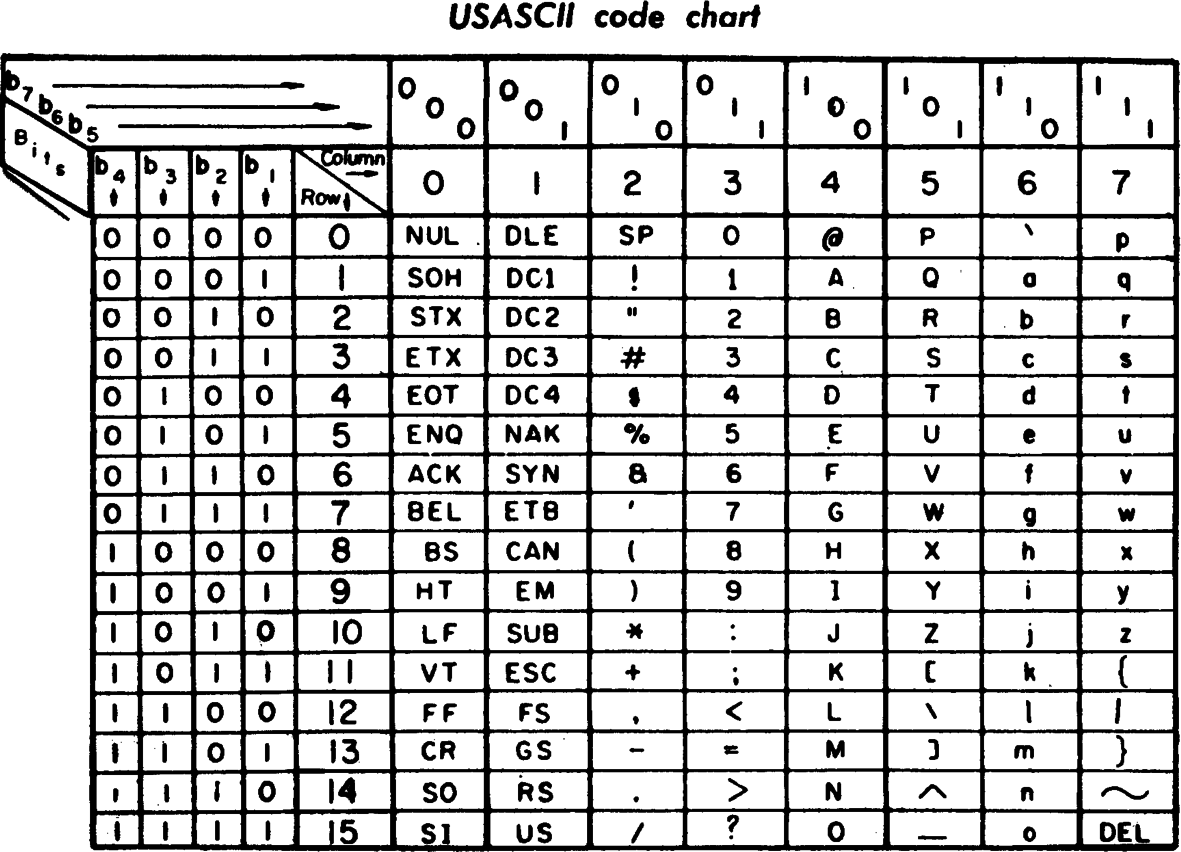
\includegraphics[width=\paperwidth]{imagens/ascii-chart}
    \par
  \end{centering}
\end{frame}

% A primeira codificação ficou conhecida como OT1 e a maior parte dos
% caracteres veio da tabela ASCII. Sintaxe para inserir acentos.
\begin{frame}[fragile]
  \frametitle{\filename{fontes.tex}}
  \huge
  \code{OT1}: Old Text 1
  \vspace{1em}

  \verb+Eur\'{i}pides+: Eur\'{i}pides
\end{frame}

% Essa abordagem tinha vários problemas.
\begin{frame}
  \frametitle{\filename{fontes.tex}}
  \huge
  Problemas da \code{OT1}:

  \begin{itemize}
    \only<1>{\item Palavras acentuadas não hifenizavam}
    \only<2>{\item Não era possível buscar por palavras acentuadas, muito menos
    copiá-las}
    \only<3>{\item E outros sistemas de escrita?}
  \end{itemize}
\end{frame}

% O problema começou a ser resolvido (para nós, falantes de português) mais de
% dez anos após o lançamento do LaTeX
\begin{frame}
  \frametitle{\filename{fontes.tex}}
  \huge
  1990 em Cork, Irlanda: nasce o \code{T1}, com 256 glifos
\end{frame}

% Quando comecei a usar LaTeX, aprendi a usar os seguintes pacotes e opções.
% Hoje, vamos aprender uma maneira melhor de fazer isso.
\begin{frame}[fragile]
  \frametitle{\filename{fontes.tex}}
  \begin{minted}[autogobble,fontsize=\LARGE,breaklines]{latex}
    \usepackage[utf8]{inputenc}
    \usepackage[T1]{fontenc}
  \end{minted}
\end{frame}

% Vamos falar sobre a diferença entre Unicode e os algorítimos de codificação
\begin{frame}
  \frametitle{\filename{fontes.tex}}
  \Huge
  \only<1>{Chega o Unicode!}
  \only<2>{Hoje com 120\,000 caracteres}
  \only<3>{Não é uma codificação, mas como uma tabela}
  \only<4>{UTF-8, UTF-16 e UTF-32 fazem o trabalho sujo}
  \only<5>{Hoje em \LaTeX, temos a codificação de fonte \code{TU}}
\end{frame}

% O pacote fontspec é carregado automaticamente pelo polyglossia, mas
% carregaremos ele mesmo assim.
\begin{frame}[fragile]
  \frametitle{\filename{fontes.tex}}
  \huge
  Aproveitar as vantagens do Unicode:

  \begin{minted}[autogobble,fontsize=\huge,breaklines]{latex}
    \usepackage{fontspec}
  \end{minted}
\end{frame}

% Exemplo do que podemos fazer usando LaTeX e Unicode. É claro, a fonte tem que
% conter os caracteres que estamos tentando usar.
\begin{frame}
  \frametitle{\filename{fontes.tex}}
  \Huge
  Εὐριπίδης — meu amigo de tantos anos — só lê Достое́вский.
\end{frame}

% Vamos aprender a acessar os diversos tipos de uma família de fontes. Vamos
% discutir com mais profundidade no exemplo e exercício.
\begin{frame}[fragile]
  \frametitle{\filename{fontes.tex}}
  \Huge
  \only<1>{Fontes vêm em famílias}
  \only<2>{\mintinline{latex}{\emph}: \emph{ênfase}}
  \only<3>{\mintinline{latex}{\textbf}: \textbf{negrito}}
  \only<4>{\mintinline{latex}{\textsc}: \textsc{Versaletes}}
  \only<5>{\mintinline{latex}{\texttt}: \texttt{teletipo}}
\end{frame}

% Tamanhos de fontes em LaTeX. Geralmente não é uma boa ideia usar eles à mão,
% pois os designers das classes de documento tomam essas decisões para nós. 
\begin{frame}[fragile]
  \frametitle{\filename{fontes.tex}}
  \large
  Tamanhos de fonte:
  \begin{multicols}{2}
    \begin{itemize}
      \item{\code{\textbackslash tiny}: 5pt}
      \item{\code{\textbackslash scriptsize}: 7pt}
      \item{\code{\textbackslash footnotesize}: 8pt}
      \item{\code{\textbackslash small}: 9pt}
      \item{\code{\textbackslash normalsize}: 10pt}
      \item{\code{\textbackslash large}: 12pt}
      \item{\code{\textbackslash Large}: 14pt}
      \item{\code{\textbackslash LARGE}: 17pt}
      \item{\code{\textbackslash huge}: 20pt}
      \item{\code{\textbackslash Huge}: 25pt}
    \end{itemize}
  \end{multicols}
\end{frame}

\begin{frame}
  \frametitle{\filename{fontes.tex}}
  \begin{quote}
    \underline{\textbf{Remember\Huge!}} \textit{The}
    \textsf{M\textbf{\LARGE O} \texttt{R}\textsl{E}} fonts \Huge you
    \tiny use \footnotesize \textbf{in} a \small \texttt{document},
    \large \textit{the} \normalsize more \textsc{readable} and
    \textsl{\textsf{beautiful} it bec\large o\Large m\LARGE e\huge s}.
  \end{quote}
\end{frame}

% Como trocar as fontes. Explicar que fontes matemáticas são outra história.
\begin{frame}[fragile]
  \frametitle{\filename{fontes.tex}}
  \Large
  Carregar fontes usando o \code{fontspec}:

  \begin{minted}[autogobble,fontsize=\Large,breaklines]{latex}
    \usepackage{fontspec}
      \setmainfont{Linux Libertine}
  \end{minted}
\end{frame}

% Fontes devem estar nos diretórios padrão. Caso não estejam, podemos
  % especificar um diret´orio:
\begin{frame}[fragile]
  \frametitle{\filename{fontes.tex}}
  \Large
  Especificar um diretório:

  \begin{minted}[autogobble,fontsize=\Large,breaklines]{latex}
    \usepackage{fontspec}
      \setmainfont{Linux Libertine}[
        Path = fonts/
      ]
  \end{minted}
\end{frame}

% Ligaduras são sequências de letras que naturalmente colidem. Por isso, são
% substituídas por outro caractere.
\begin{frame}
  \frametitle{\filename{fontes.tex}}
  \Huge
  Linux Libertine e ligaduras

  \fontspec{Linux Libertine}{
    affair\qquad fjord\qquad flor\\
    af\mbox{}fair\qquad f\mbox{}jord\qquad f\mbox{}lor
  }
\end{frame}

% Antes do exercício, vamos rever os conceitos que discutimos de maneira
% prática.
\begin{frame}
  \frametitle{\filename{fontes.tex}}
  \Huge
  Demonstrar ideias em \filename{fontes.tex}
\end{frame}

% Resolver o exercício fontes-exercicio.tex.
\begin{frame}
  \frametitle{\filename{fontes.tex}}
  \Huge
  Resolver \filename{fontes-exercicio.tex}
\end{frame}

% layouts-pagina.tex %%%%%%%%%%%%%%
\begin{frame}[standout]
  \Huge
   \filename{layouts-pagina.tex}
\end{frame}

% Vamos mudar a opção de classe de onecolumn para twocolumn e carregar o pacote
% showframe.
\begin{frame}
  \frametitle{\filename{layouts-pagina.tex}}
  \huge
  \only<1>{Copiar solução de \filename{fontes-exercio.tex} como
  \filename{layouts-pagina.tex}}
  \only<2>{Mudar para \code{twocolumn}, carregar o pacote \code{showframe}}
\end{frame}

% Na folha A4, apenas uma coluna coluna de texto é difícil de ler com margens
% curtas. Mas usar margens grandes desperdiça papel.
\begin{frame}
  \frametitle{\filename{layouts-pagina.tex}}
  \huge
  \code{onecolumn}: margens grandes demais

  \code{twocolumn}: nem sempre podemos
\end{frame}

% Soluções para o problema do tamanho da coluna de texto vs margens
\begin{frame}
  \frametitle{\filename{layouts-pagina.tex}}
  \huge
  Soluções:
  \begin{itemize}
    \only<1>{\item Colunas}
    \only<2>{\item \code{fullpage}}
    \only<3>{\item \code{fullpage} e entrelinhas maiores}
  \end{itemize}
\end{frame}

% Se decidirmos usar o pacote fullpage, é uma boa ideia aumentar o espaçamento
% entre as linhas.
\begin{frame}
  \frametitle{\filename{layouts-pagina.tex}}
  \huge
  Pacote \code{setspace}:

  \begin{itemize}
    \item \code{\textbackslash singlespacing}
    \item \code{\textbackslash onehalfspacing}
    \item \code{\textbackslash doublespacing}
  \end{itemize}
\end{frame}

% Outro fator que influencia o layout da página é seu estilo. Estes são os três
% comandos básicos e estilos que podemos escolher.
\begin{frame}
  \frametitle{\filename{layouts-pagina.tex}}
  \huge
  \code{\textbackslash pagestyle} e \code{\textbackslash thispagestyle}

  \begin{itemize}
    \item \code{empty}
    \item \code{plain}
    \item \code{headings}
  \end{itemize}
\end{frame}

% Outro fator que influencia o layout da página é seu estilo. Estes são os três
% comandos básicos e estilos que podemos escolher.
\begin{frame}
  \frametitle{\filename{layouts-pagina.tex}}
  \huge
  Demonstração em \filename{layouts-pagina.tex}
\end{frame}

% Exercício: faremos um certificado de conclusão do curso
\begin{frame}
  \frametitle{\filename{layouts-pagina-exercicio.tex}}
  \Huge
  Certificado de conclusão
\end{frame}

% Uma ideia de como ele poderia ficar
\begin{frame}[plain]
  \begin{center}
    {\huge\textbf{OpenSanca}}\\[2em]
    {\LARGE\textsc{Certificado}}
  \end{center}

    \noindent Certificamos que Tal Pessoa da Silva participou de um curso em
    nosso grupo no dia 28 de maio de 2016 e está qualificado para editar textos
    em \LaTeX.

    \vfill
    \begin{flushright}
      \emph{Os Organizadores}\\
      \emph{OpenSanca}\\
    \end{flushright}
\end{frame}

% Começar nosso certificado de conclusão de curso
\begin{frame}
  \frametitle{\filename{layouts-pagina.tex}}
  \Huge
  Resolver \filename{layouts-pagina-exercicio.tex}
\end{frame}

% posicao-texto.tex %%%%%%%%%%%%%%
\begin{frame}[standout]
  \Huge
   \filename{posicao-texto.tex}
\end{frame}

% Nosso certificado pode ter ficado legal, mas poderia ser melhor ainda se
% ajustarmos o texto em relação à página.
\begin{frame}
  \frametitle{\filename{posicao-texto.tex}}
  \Huge
  Problemas com o certificado?
\end{frame}

% Antes de controlar a posição do texto, temos que entender o que é um
% ambiente.
\begin{frame}[fragile]
  \frametitle{\filename{posicao-texto.tex}}
  \Huge
  Ambientes:

  \begin{minted}[autogobble,fontsize=\Huge,breaklines]{latex}
    \begin{ambiente}
      …
    \end{ambiente}
  \end{minted}
\end{frame}

% Três ambientes para controlar posição.
\begin{frame}[fragile]
  \frametitle{\filename{posicao-texto.tex}}
  \Large
  Ambientes \code{center}, \code{flushleft} e \code{flushright}

  % Código:
  \begin{minted}[autogobble,fontsize=\Large,breaklines]{latex}
    \begin{center}
      Este texto será centralizado.
    \end{center}
  \end{minted}

  % Resultado:
  \begin{center}
    Este texto será centralizado.
  \end{center}
\end{frame}

% Ainda podemos controlar o espaço dentro de uma linha.
\begin{frame}[fragile]
  \frametitle{\filename{posicao-texto.tex}}
  \Huge
  \mintinline{latex}{\hspace{comprimento}}
\end{frame}

% Por exemplo, um espaço de 1,5cm:
\begin{frame}[fragile]
  \frametitle{\filename{posicao-texto.tex}}
  \LARGE
  \begin{minted}[autogobble,fontsize=\LARGE,breaklines]{latex}
    Essa frase\hspace{1.5cm} está esticada.
  \end{minted}
  \vspace{1em}

  Essa frase\hspace{1.5cm} está esticada.
\end{frame}

% O LaTeX aceita uma série de unidades
\begin{frame}[fragile]
  \frametitle{\filename{posicao-texto.tex}}
  \LARGE
  Unidades que o \LaTeX{} conhece:

  \begin{multicols}{2}
    \begin{itemize}
      \item\code{mm}
      \item\code{cm}
      \item\code{in}
      \item\code{pt}
      \item\code{em}
      \item\code{ex}
      \item\mintinline{latex}{\textheight}
      \item\mintinline{latex}{\textwidth}
      \item\mintinline{latex}{\pageheight}
      \item\mintinline{latex}{\pageheight}
    \end{itemize}
  \end{multicols}
\end{frame}

% O comando \hfill preenche todo o espaço disponível
\begin{frame}[fragile]
  \frametitle{\filename{posicao-texto.tex}}
  \LARGE
  \mintinline{latex}{Começo\hfill meio\hfill fim}
  \vspace{1em}

  Começo\hfill meio\hfill fim
\end{frame}

% E, finalmente, existem os comandos \vspace e \hfill
\begin{frame}[fragile]
  \frametitle{\filename{posicao-texto.tex}}
  \huge
  Comandos análogos:

  \mintinline{latex}{\vspace{comprimento}}
  \vspace{1em}

  \mintinline{latex}{\vfill}
\end{frame}

% Exercício: terminar o certificado que começamos antes
\begin{frame}
  \frametitle{\filename{posicao-texto.tex}}
  \Huge
  Resolver \filename{posicao-texto-exercicio.tex}
\end{frame}

% listas.tex %%%%%%%%%%%%%%
\begin{frame}[standout]
  \Huge
  \filename{listas.tex}
\end{frame}

% Três tipos de listas inclusos por padrão
\begin{frame}
  \frametitle{\filename{listas.tex}}
  \Huge
  Ambientes: \code{itemize, enumerate} e \code{description}
\end{frame}

% Anatomia de uma lista
\begin{frame}[fragile]
  \frametitle{\filename{listas.tex}}
  \LARGE
  Ingredientes para carbonara:

  \begin{minted}[autogobble,fontsize=\Large,breaklines]{latex}
    \begin{itemize}
      \item Bacon
      \item Macarrão
      \item Ovos
      \item Parmesão
      \item Pimenta-do-reino
    \end{itemize}
  \end{minted}
\end{frame}

% Exercício: completar a receita de panqueca com os ingredientes corretos.
\begin{frame}
  \frametitle{\filename{listas.tex}}
  \Huge
  Resolver \filename{listas-exercicio.tex}
\end{frame}

% Lista de ingredientes que os participantes devem colocar na receita. Notar a
% palavra ingrediente, o número sequencial e o parênteses.
\begin{frame}
  \frametitle{\filename{listas.tex}}
  \large
  \begin{enumerate}[{Ingrediente} 1)]
    \item 190g de farinha
    \item 25g de açúcar
    \item 10g de fermento químico em pó
    \item 3g de sal\\[1em] … texto …\\
    \item 25g de manteiga\\[1em] … texto …\\
    \item 330g de leite
    \item 80g de ovos
  \end{enumerate}
\end{frame}

% Existem mais listas no arquivo listas.tex
\begin{frame}
  \frametitle{\filename{listas.tex}}
  \Huge
  Aprenderemos mais em \filename{listas.tex}
\end{frame}

% citacoes-versos.tex %%%%%%%%%%%%%%
\begin{frame}[standout]
  \Huge
  \filename{citacoes-versos.tex}
\end{frame}

% Ambientes quote e quotation
\begin{frame}
  \frametitle{\filename{citacoes-versos.tex}}
  \Huge
  Ambientes: \code{quote} e \code{quotation}
\end{frame}

% Exemplo de uso do ambiente quote
\begin{frame}[fragile]
  \frametitle{\filename{citacoes-versos.tex}}
  \Large
  \begin{minted}[autogobble,fontsize=\Large,breaklines]{latex}
  \begin{quote}
    Não entre em pânico!\hfill (Douglas Adams)
  \end{quote}
  \end{minted}
  \vspace{1em}

  \begin{quote}
    Não entre em pânico!\hfill (Douglas Adams)
  \end{quote}
\end{frame}

% Exemplo de uso do ambiente verse
\begin{frame}[fragile]
  \frametitle{\filename{citacoes-versos.tex}}
  \begin{minted}[autogobble,fontsize=\large,breaklines]{latex}
    \begin{verse}
      O vinho dá-te o calor que não tens;\\
      suaviza o jugo do passado e te alivia\\
      das brumas do futuro; inunda-te de luz\\
      e te liberta desta prisão.
      \flushright
      (Omar Khayyam)
    \end{verse}
  \end{minted}
\end{frame}

% Output do comando anterior
\begin{frame}
  \frametitle{\filename{citacoes-versos.tex}}
  \Large
  \begin{verse}
    O vinho dá-te o calor que não tens;\\
    suaviza o jugo do passado e te alivia\\
    das brumas do futuro; inunda-te de luz\\
    e te liberta desta prisão.
    \flushright
    (Omar Khayyam)
  \end{verse}
\end{frame}

% tabelas.tex %%%%%%%%%%%%%%
\begin{frame}[standout]
  \Huge
  \filename{tabelas.tex}
\end{frame}

% Exemplo simples de tabela com o ambiente tabular
\begin{frame}[fragile]
  \frametitle{\filename{tabelas.tex}}
  \Large
  Exemplo do ambiente \code{tabular}:
  \vspace{1em}

  \begin{minipage}{.65\textwidth}
    \begin{minted}[autogobble,fontsize=\large,breaklines]{latex}
      \begin{tabular}{lcr}
        1 & 2 & 3\\
        4 & 5 & 6\\
        7 & 8 & 9
      \end{tabular}
    \end{minted}
  \end{minipage}
  \hspace{.05\textwidth}
  \begin{minipage}{.25\textwidth}
    \begin{tabular}{lcr}
      1 & 2 & 3\\
      4 & 5 & 6\\
      7 & 8 & 9
    \end{tabular}
  \end{minipage}
\end{frame}

% Com mais alguns detalhes como linhas verticais e horizontais
\begin{frame}[fragile]
  \frametitle{\filename{tabelas.tex}}
  \Large
  Linhas horizontais e verticais:
  \vspace{1em}

  \begin{minipage}{.65\textwidth}
    \begin{minted}[autogobble,fontsize=\large,breaklines]{latex}
      \begin{tabular}{l|c|r}
        \hline
        1 & 2 & 3\\
        4 & 5 & 6\\
        7 & 8 & 9\\
        \hline
      \end{tabular}
    \end{minted}
  \end{minipage}
  \hspace{.05\textwidth}
  \begin{minipage}{.25\textwidth}
    \begin{tabular}{l|c|r}
      \hline
      1 & 2 & 3\\
      4 & 5 & 6\\
      7 & 8 & 9\\
      \hline
    \end{tabular}
  \end{minipage}
\end{frame}

% O espaço em branco deixa o texto respirar e evita a tirania das linhas retas.
% Essa citação do Bringhurst é fantástica.
\begin{frame}
  \frametitle{\filename{tabelas.tex}}
  \large
  \begin{quote}
    Assim como o texto, as tabelas ficam canhestras quando abordadas de forma
    puramente técnica. Boas soluções tipográficas não costumam surgir em resposta
    a perguntas do tipo “Como posso enfiar essa quantidade de caracteres naquele
    tanto de espaço?”.\\\hfill (Robert Bringhurst, \emph{Elementos do Estilo
    Tipográfico)}
  \end{quote}
\end{frame}

% Vejamos alguns exemplos de tabela em tabelas.tex.
\begin{frame}
  \frametitle{\filename{tabelas.tex}}
  \Huge
  Vejamos \filename{tabelas.tex}
\end{frame}

% Vamos revisar o que aprendemos no exemplo.
\begin{frame}[fragile]
  \frametitle{\filename{tabelas.tex}}
  \Huge
  Aprendemos:

  \begin{itemize}
    \only<1>{\item \code{tabular}}
    \only<1>{\item tipografia da tabela}
    \only<2>{\item quebras de linhas}
    \only<2>{\item \code{booktabs}}
    \only<3>{\item \mintinline{latex}{\multicolumn}}
    \only<3>{\item \code{longtable}}
  \end{itemize}
\end{frame}

% Exercício: formatar uma lista em CSV
\begin{frame}
  \frametitle{\filename{tabelas.tex}}
  \Huge
  Resolver: \filename{tabelas-exercicio.tex}
\end{frame}

% Temos declarado exatamente onde desejamos que a tabela fique, mas essa
% abordagem nem sempre é boa, porque interrompe o fluxo do texto. Vamos
% aprender mais sobre os ambientes do tipo float.
\begin{frame}
  \frametitle{\filename{tabelas.tex}}
  \Huge
  \only<1>{Ambiente \code{tabular} coloca a tabela após o texto}
  \only<2>{Padrão profissional: \emph{floats}}
  \only<3>{Dois floats: \code{table} e \code{figure}}
\end{frame}

% A sintaxe do ambiente table
\begin{frame}[fragile]
  \frametitle{\filename{tabelas.tex}}
  \Large
  Sintaxe de \code{table}:
  \vspace{1em}

    \begin{minted}[autogobble,fontsize=\large,breaklines]{latex}
      \begin{table}[posição]
        …
      \end{table}
    \end{minted}
\end{frame}

% Exemplo, com os comandos \centering, \caption e \label.
\begin{frame}[fragile]
  \frametitle{\filename{tabelas.tex}}
  \Large
  Veja a tabela~\ref{tab:numerosUmNove}:

  \begin{minipage}{.65\textwidth}
    \begin{minted}[autogobble,fontsize=\large,breaklines]{latex}
    \begin{table}
      \centering
      \begin{tabular}{lcr}
      1 & 2 & 3\\
      4 & 5 & 6\\
      7 & 8 & 9
      \end{tabular}
      \caption{Números de 1 a 9}
      \label{tab:numerosUmNove}
    \end{table}
    \end{minted}
  \end{minipage}
  \hspace{.05\textwidth}
  \begin{minipage}{.25\textwidth}
    \begin{table}
      \centering
      \begin{tabular}{lcr}
        1 & 2 & 3\\
        4 & 5 & 6\\
        7 & 8 & 9
      \end{tabular}
      \caption{Números de 1 a 9}
      \label{tab:numerosUmNove}
    \end{table}
  \end{minipage}
\end{frame}

% Voltaremos ao arquivo anterior para brincar com esses conceitos e
% referências cruzadas.
\begin{frame}
  \frametitle{\filename{tabelas.tex}}
  \Huge
  Voltemos a \filename{tabelas.tex}
\end{frame}

% Exercício: uma tabela do zero, usando o ambiente table e referenciando a
% tabela num parágrafo anterior.
\begin{frame}
  \frametitle{\filename{tabelas.tex}}
  \Huge
  Resolver: \filename{tabelas-questionario-exercicio.tex}
\end{frame}

\begin{frame}
  \frametitle{\filename{tabelas.tex}}
  \Huge
  Pacote \code{tabularx}
\end{frame}

\begin{frame}
  \frametitle{\filename{tabelas.tex}}
  \Huge
  Veja o documento \filename{fala.md} para mais ferramentas
\end{frame}

% imagens.tex %%%%%%%%%%%%%%
\begin{frame}[standout]
  \Huge
  \filename{imagens.tex}
\end{frame}

% Para inserir imagens, precisamos carregar o pacote graphicx
\begin{frame}
  \frametitle{\filename{imagens.tex}}
  \Huge
  Pacote \code{graphicx}
\end{frame}

% O pacote graphics nos dá acesso ao comando \includegraphics, que aceita uma
% série de opções. Não discutiremos todas em nosso workshop, mas as mais úteis
% são width, height, scale e keepaspectratio.
\begin{frame}[fragile]
  \frametitle{\filename{imagens.tex}}
  \Large
  \mintinline{latex}{\includegraphics[opções]{imagem}}
  \vspace{1em}

  Algumas opções:
  \begin{itemize}
    \item \code{width} e \code{height}
    \item \code{scale}
    \item \code{keepaspectratio} (bool)
  \end{itemize}
\end{frame}

% Geralmente, usamos o comando \includegraphics com o ambiente figure, que é
% bastante parecido com o ambiente table, que acabamos de estudar.
\begin{frame}[fragile]
  \frametitle{\filename{imagens.tex}}
  \Large
  Ambiente \code{figure}:

    \begin{minted}[autogobble,fontsize=\Large,breaklines]{latex}
    \begin{figure}[h]
      \centering
      \includegraphics{imagem}
      \caption{Exemplo de imagem}
      \label{fig:imagem}
    \end{figure}
    \end{minted}
\end{frame}

% Demonstrar os conceitos usando o arquivo imagens.tex.
\begin{frame}
  \frametitle{\filename{imagens.tex}}
  \Huge
  Estudar \filename{imagens.tex}
\end{frame}

% Exercício: colocar figuras no questionário que fizemos anteriormente.
\begin{frame}
  \frametitle{\filename{imagens.tex}}
  \Huge
  Resolver \filename{imagens-exercicio.tex}
\end{frame}

% matematica.tex %%%%%%%%%%%%%%
\begin{frame}[standout]
  \Huge
  \filename{matematica.tex}
\end{frame}

% Até agora, estávamos no modo de texto. No modo de matemática, o modo como o
% LaTeX interpreta o que escrever é diferente. Além disso, o modo de matemática
% é dividido em dois tipos: inline e displayed
\begin{frame}
  \frametitle{\filename{matematica.tex}}
  \Huge
  \only<1>{Modo de texto vs.\\ modo de matemática}
  \only<2>{Modo de matemática: \emph{inline} e \emph{displayed}}
\end{frame}

% Existem três ambientes para acessar o modo de matemática.
\begin{frame}[fragile]
  \frametitle{\filename{matematica.tex}}
  \huge
  Três ambientes:\\

  \only<1>{\mintinline{latex}{math} ou \mintinline{latex}{\( … \)}}
  \only<2>{\mintinline{latex}{displaymath} ou \mintinline{latex}{\[ … \]}}
  \only<3>{\mintinline{latex}{equation}}
\end{frame}

% Há uma infinidade de comandos, pacotes e técnicas para aprender. Cobriremos o
% básico.
\begin{frame}
  \frametitle{\filename{matematica.tex}}
  \Huge
  Cobriremos o básico!
\end{frame}

% Símbolos em modo matemático
\begin{frame}[fragile]
  \frametitle{\filename{matematica.tex}}
  \huge
  \mintinline{latex}{2 \times 2 = 4}

  \[ 2 \times 2 = 4 \]
\end{frame}

% Letras gregas
\begin{frame}[fragile]
  \frametitle{\filename{matematica.tex}}
  \huge
  \mintinline{latex}{\alpha, \beta, \pi}

  \[ \alpha, \beta, \pi \]
\end{frame}

% Operadores
\begin{frame}[fragile]
  \frametitle{\filename{matematica.tex}}
  \begin{minted}[autogobble,fontsize=\Large,breaklines]{latex}
    \cos (2\theta) = \cos^2 \theta - \sin^2 \theta
  \end{minted}

  \huge
  \[ \cos (2\theta) = \cos^2 \theta - \sin^2 \theta \]
\end{frame}

% Potências e subscritos
\begin{frame}[fragile]
  \frametitle{\filename{matematica.tex}}
  \Large

  \begin{minipage}{.65\textwidth}
    \begin{minted}[autogobble,fontsize=\Large,breaklines]{latex}
      2^8
      a_b
      2^{32}
      f(n) = 4n + n^2
    \end{minted}
  \end{minipage}
  \begin{minipage}{.25\textwidth}
    \[ 2^8 \]

    \[ a_b \]

    \[ 2^{32} \]

    \[ f(n) = 4n + n^2 \]
  \end{minipage}
\end{frame}

% Frações
\begin{frame}[fragile]
  \frametitle{\filename{matematica.tex}}
  \Large
  \begin{minted}[autogobble,fontsize=\large,breaklines]{latex}
    F = G \frac{m_1 m_2}{d^2}
    \frac{\frac{1}{x}+\frac{1}{y}}{y-z}
  \end{minted}

  \[ F = G \frac{m_1 m_2}{d^2} \]

  \[ \frac{\frac{1}{x}+\frac{1}{y}}{y-z} \]
\end{frame}

% Raízes
\begin{frame}[fragile]
  \frametitle{\filename{matematica.tex}}
  \Large
  \begin{minipage}{.55\textwidth}
    \begin{minted}[autogobble,fontsize=\Large,breaklines]{latex}
      \sqrt{10^2} = 9
      \sqrt[3]{\frac{a}{b}}
    \end{minted}
  \end{minipage}
  \begin{minipage}{.35\textwidth}
    \[ \sqrt{10^2} = 9 \]

    \[ \sqrt[3]{\frac{a}{b}} \]
  \end{minipage}
\end{frame}

% Exercício: reproduza essa equação em matematica-exercicio.tex
\begin{frame}
  \frametitle{\filename{matematica-exercicio.tex}}
  \Large
  Reproduza em \filename{matematica-exercicio.tex}:

  \huge
  \begin{equation}
    x = \frac{-b \pm \sqrt{b^2 - 4ac}}{2a}
  \end{equation}
\end{frame}

% tipografia.tex %%%%%%%%%%%%%%
\begin{frame}[standout]
  \Huge
  \filename{tipografia.tex}
\end{frame}

% Um dos principais motivos para se usar o LaTeX é justamente sua qualidade
% tipográfica.
\begin{frame}
  \frametitle{\filename{tipografia.tex}}
  \Huge
  \begin{quote}
    A tipografia que tem algo a dizer aspira a ser uma espécie de estátua
    transparente.\hfill(Robert Bringhurst)
  \end{quote}
\end{frame}

% Pontuação: quatro traços diferentes
\begin{frame}
  \frametitle{\filename{tipografia.tex}}
  \Huge
  \begin{itemize}
    \item O travessão: —
    \item A meia-risca: –
    \item O hífen: -
    \item O sinal de menos: \( - \)
  \end{itemize}
\end{frame}

% O travessão
\begin{frame}[fragile]
  \frametitle{\filename{tipografia.tex}}
  \LARGE
  Travessão: —

  \mintinline{latex}{--- Como assim? --- Ela disse.}

  --- Como assim? --- Ela disse.
\end{frame}

% A meia-risca
\begin{frame}[fragile]
  \frametitle{\filename{tipografia.tex}}
  \LARGE
  Meia-risca: – 

  \mintinline{latex}{páginas 10--15}

  páginas 10--15
\end{frame}

% O hífen
\begin{frame}[fragile]
  \frametitle{\filename{tipografia.tex}}
  \LARGE
  Hífen: -

  \mintinline{latex}{guarda-chuva}

  guarda-chuva
\end{frame}

% Sinal de menos
\begin{frame}[fragile]
  \frametitle{\filename{tipografia.tex}}
  \LARGE
  Sinal de menos: \( - \)

  \mintinline{latex}{\( 15 - 15 \)}

  \( 15 - 15 \)
\end{frame}

% Aspas: diferença entre aspas retas e curvas
\begin{frame}
  \frametitle{\filename{tipografia.tex}}
  \huge
  \begin{itemize}
    \item Aspas retas: "Olá, mundo".
    \item Aspas curvas: “Olá, mundo".
  \end{itemize}
\end{frame}

% Sintaxe: `` e '' ou “”
\begin{frame}[fragile]
  \frametitle{\filename{tipografia.tex}}
  \Huge
  \mintinline{latex}{``Olá, mundo''.}
  \mintinline{latex}{“Olá, mundo”.}

  ``Olá, mundo''.\\
  “Olá, mundo”.
\end{frame}

% Reticências
\begin{frame}[fragile]
  \frametitle{\filename{tipografia.tex}}
  \Huge
  \mintinline{latex}{Olá, mundo\ldots}

  Olá, mundo\ldots
\end{frame}

% Espaços duros
\begin{frame}[fragile]
  \frametitle{\filename{tipografia.tex}}
  \LARGE
  Espaços duros: \verb+~+\\

  % Sem espaços duros
  \only<1>{
    \begin{center}
      \fbox{
        \begin{minipage}{.5\textwidth}
          O Sr. Roberto disser que a Sra. Eduarda quer 100 páginas até o dia 5.
          Às 9 eu só havia terminado 60!
        \end{minipage}
      }
    \end{center}
  }

  % Com espaços duros
  \only<2>{
    \begin{center}
      \fbox{
        \begin{minipage}{.5\textwidth}
          O Sr.~Roberto disser que a Sra.~Eduarda quer~100 páginas até o dia~5.
          Às~9 eu só havia terminado~60!
        \end{minipage}
      }
    \end{center}
  }
\end{frame}

% A classe memoir vem com várias melhorias por padrão.
\begin{frame}
  \frametitle{\filename{tipografia.tex}}
  \Huge
  Recomendação: a classe \code{memoir}
\end{frame}

% Textos bilíngues
\begin{frame}
  \frametitle{\filename{tipografia.tex}}
  \Huge
  Textos com várias línguas são possíveis
\end{frame}

% Macros
\begin{frame}
  \frametitle{\filename{tipografia.tex}}
  \Huge
  Use macros para textos mais semânticos
\end{frame}

% Macros
\begin{frame}
  \frametitle{\filename{tipografia.tex}}
  \Huge
  Pacote \code{minted}: exemplos de código.
\end{frame}

% abntex2.tex %%%%%%%%%%%%%%
\begin{frame}[standout]
  \Huge
  \filename{abntex2.tex}
\end{frame}

\begin{frame}
  \frametitle{\filename{abntex2.tex}}
  \large
  \begin{quote}
    O abnTeX2, evolução do abnTeX (ABsurd Norms for TeX), é uma suíte para
    LaTeX que atende os requisitos das normas da ABNT (Associação Brasileira de
    Normas Técnicas) para elaboração de documentos técnicos e científicos
    brasileiros, como artigos científicos, relatórios técnicos, trabalhos
    acadêmicos como teses, dissertações, projetos de pesquisa e outros
    documentos do gênero.
  \end{quote}
\end{frame}

% O abnTeX2 implementa muitos novos comandos, que veremos na prática.
\begin{frame}
  \frametitle{\filename{abntex2.tex}}
  \Huge
  Implementa novos comandos
\end{frame}

% Alguns exemplos de comandos que o abnTeX2 traz
\begin{frame}
  \frametitle{\filename{abntex2.tex}}
  \Huge
  \begin{itemize}
    \item\mintinline{latex}{\titulo}
    \item\mintinline{latex}{\autor}
    \item\mintinline{latex}{\imprimircapa}
    \item\mintinline{latex}{citacao} (ambiente)
  \end{itemize}
\end{frame}

\begin{frame}
  \frametitle{\filename{abntex2.tex}}
  \Huge
  A norma regulamenta a organização dos textos
\end{frame}

\begin{frame}
  \frametitle{\filename{abntex2.tex}}
  \Huge
  Manual do abnTeX2: \url{abntex.net.br}
\end{frame}

% Vejamos um exemplo de documento. Vamos fazer um live coding!
\begin{frame}
  \frametitle{\filename{abntex2.tex}}
  \Huge
  Exemplo: \filename{abntex2.tex}
\end{frame}

% abntex2-example.bib %%%%%%%%%%%%%%
\begin{frame}[standout]
  \Huge
  \filename{abntex2-example.bib}
\end{frame}

% O BibTeX tem dois arquivos principais
\begin{frame}
  \frametitle{\filename{abntex2-example.bib}}
  \Huge
  \hologo{BibTeX}: database (\code{bib}) e estilo (\code{bst})
\end{frame}

% Um exemplo de entrada bibliográfica
\begin{frame}[fragile]
  \frametitle{\filename{abntex2-example.bib}}
  \Huge
  \code{bib}:

  \begin{minted}[autogobble,fontsize=\large,breaklines]{latex}
    @article{greenwade93,
      author  = "George D. Greenwade",
      title   = "The {C}omprehensive {T}ex {A}rchive {N}etwork ({CTAN})",
      year    = "1993",
      journal = "TUGBoat",
      volume  = "14",
      number  = "3",
      pages   = "342--351"
    }
  \end{minted}
\end{frame}

% No local desejado, colocamos a bibliografia
\begin{frame}[fragile]
  \frametitle{\filename{abntex2-example.bib}}
  \LARGE
  \verb+\bibliography{arquivo}+
\end{frame}

% Para citar, basta usar um desses comandos
\begin{frame}[fragile]
  \frametitle{\filename{abntex2-example.bib}}
  \LARGE
  \verb+\cite[p.~20]{greenwade93}+

  \verb+\citeonline[p.~20]{greenwade93}+
\end{frame}

% Mais um live coding!
\begin{frame}
  \frametitle{\filename{abntex2-example.bib}}
  \Huge
  Exemplo: \filename{abntex2-example.bib}
\end{frame}

\begin{frame}[standout]
  \Huge
  Obrigado!
\end{frame}

\end{document}
